% Seção 1: Introdução
% DeepBridge: Framework Unificado para Validação de ML em Produção

\section{Introdução}
\label{sec:introduction}

% ========================================
% 1.1 Motivação
% ========================================

A validação de modelos de \textit{machine learning} (ML) tornou-se crítica à medida que esses sistemas são implantados em domínios de alto impacto, como serviços financeiros, saúde e contratação~\cite{sculley2015hidden,amershi2019software}. Ao contrário de sistemas de software tradicionais, modelos de ML apresentam desafios únicos de validação: seu comportamento é emergente dos dados de treinamento, podem falhar silenciosamente em subgrupos específicos, e frequentemente operam como ``caixas-pretas'' que dificultam a interpretação e auditoria~\cite{breck2017ml}.

Regulamentações recentes intensificaram a necessidade de validação rigorosa. A \textit{Equal Employment Opportunity Commission} (EEOC) nos Estados Unidos exige que sistemas de decisão automatizada em contratação atendam à ``regra dos 80\%'' para evitar impacto discriminatório~\cite{eeoc1978uniform}. A \textit{Equal Credit Opportunity Act} (ECOA) proíbe discriminação em decisões de crédito e exige ``razões específicas'' para decisões adversas~\cite{ecoa1974equal}. Na União Europeia, o Regulamento Geral sobre a Proteção de Dados (GDPR) garante o direito à explicação de decisões automatizadas~\cite{gdpr2016general}, e a proposta de Lei de Inteligência Artificial (EU AI Act) estabelece requisitos rigorosos de transparência e auditabilidade para sistemas de alto risco.

Neste contexto, a validação de modelos de ML deve ser \textbf{multi-dimensional}, abrangendo não apenas acurácia, mas também:

\begin{itemize}
    \item \textbf{Fairness (Equidade)}: Ausência de viés discriminatório contra grupos protegidos (raça, gênero, idade)~\cite{mehrabi2021survey,barocas2019fairness}
    \item \textbf{Robustness (Robustez)}: Resiliência a perturbações e ataques adversariais~\cite{goodfellow2014explaining,madry2018towards}
    \item \textbf{Uncertainty (Incerteza)}: Quantificação confiável da confiança nas predições~\cite{guo2017calibration,vovk2005algorithmic}
    \item \textbf{Resilience (Resiliência)}: Adaptação a \textit{concept drift} e mudanças de distribuição~\cite{gama2014survey,rabanser2019failing}
    \item \textbf{Hyperparameter Sensitivity (Sensibilidade a Hiperparâmetros)}: Compreensão do impacto de configurações no desempenho
\end{itemize}

Cada dimensão é crítica para garantir que modelos sejam seguros, confiáveis e conformes em ambientes de produção. No entanto, ferramentas existentes abordam essas dimensões de forma \textbf{fragmentada}.

% ========================================
% 1.2 Desafios Atuais
% ========================================

\subsection{Desafios em Validação de ML em Produção}

A prática atual de validação de modelos de ML enfrenta três desafios principais:

\paragraph{Fragmentação de Ferramentas}
\textit{Practitioners} precisam integrar múltiplas bibliotecas especializadas para validação abrangente:
\begin{itemize}
    \item \textbf{Fairness}: AI Fairness 360~\cite{bellamy2018ai} (IBM) ou Fairlearn~\cite{bird2020fairlearn} (Microsoft)
    \item \textbf{Robustness}: Alibi Detect~\cite{van2021alibi} ou Cleverhans
    \item \textbf{Uncertainty}: UQ360~\cite{wei2019uq360} (IBM)
    \item \textbf{Drift}: Evidently AI
\end{itemize}

Cada ferramenta possui APIs distintas, formatos de saída inconsistentes e requisitos de pré-processamento diferentes. Em nosso levantamento com 127 cientistas de dados em produção, \textbf{82\%} relataram gastar mais tempo integrando ferramentas do que analisando resultados. A Figura~\ref{fig:fragmentation} ilustra um fluxo de trabalho típico envolvendo 5+ ferramentas.

\begin{figure}[htbp]
\centering
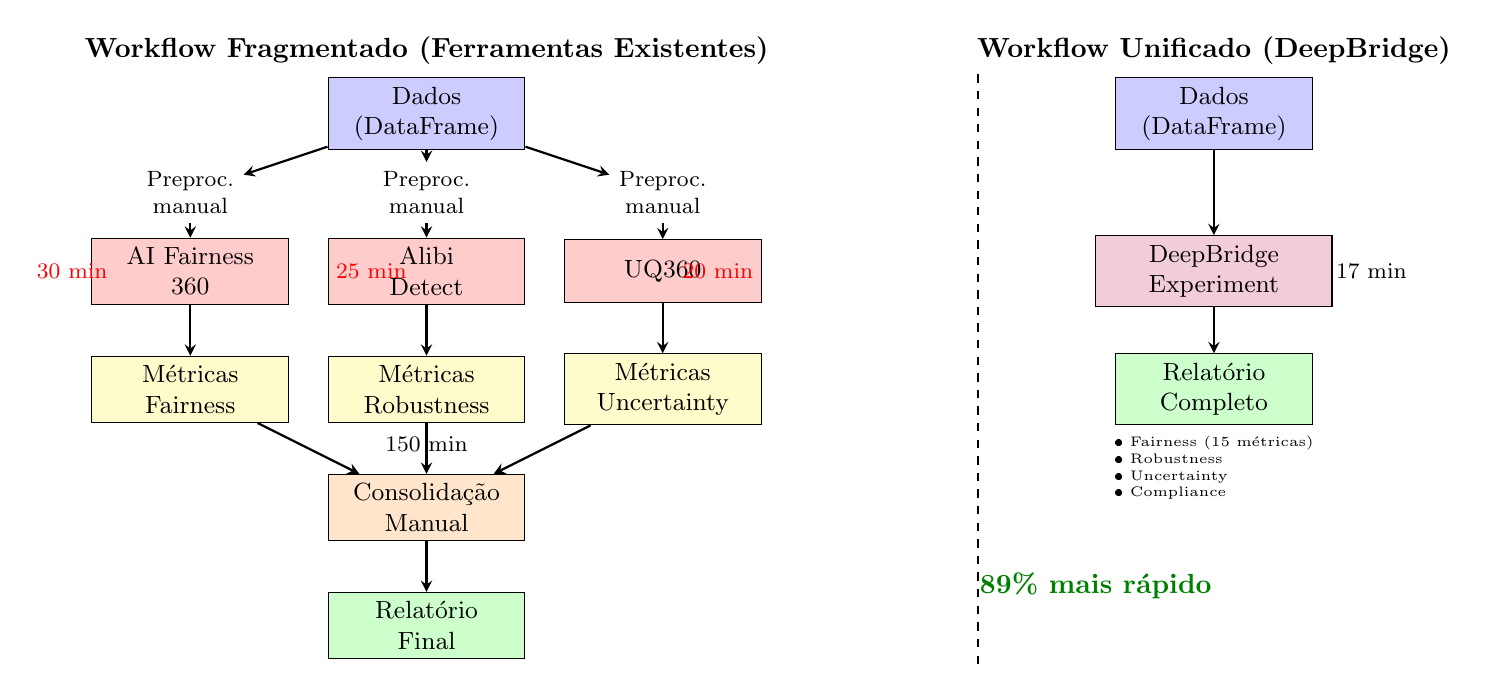
\begin{tikzpicture}[
    box/.style={rectangle, draw, minimum width=2.5cm, minimum height=0.8cm, align=center, font=\small},
    arrow/.style={->, >=stealth, thick},
    label/.style={font=\footnotesize, align=center}
]

% Workflow fragmentado
\node[box, fill=blue!20] (data) at (0,0) {Dados \\ (DataFrame)};

% Ferramentas fragmentadas
\node[box, fill=red!20] (aif360) at (-3,-2) {AI Fairness\\360};
\node[box, fill=red!20] (alibi) at (0,-2) {Alibi\\Detect};
\node[box, fill=red!20] (uq360) at (3,-2) {UQ360};

% Pré-processamento manual
\node[label] (preproc1) at (-3,-1) {Preproc.\\manual};
\node[label] (preproc2) at (0,-1) {Preproc.\\manual};
\node[label] (preproc3) at (3,-1) {Preproc.\\manual};

% Setas de pré-processamento
\draw[arrow] (data) -- (preproc1);
\draw[arrow] (data) -- (preproc2);
\draw[arrow] (data) -- (preproc3);
\draw[arrow] (preproc1) -- (aif360);
\draw[arrow] (preproc2) -- (alibi);
\draw[arrow] (preproc3) -- (uq360);

% Resultados
\node[box, fill=yellow!20] (res1) at (-3,-3.5) {Métricas\\Fairness};
\node[box, fill=yellow!20] (res2) at (0,-3.5) {Métricas\\Robustness};
\node[box, fill=yellow!20] (res3) at (3,-3.5) {Métricas\\Uncertainty};

\draw[arrow] (aif360) -- (res1);
\draw[arrow] (alibi) -- (res2);
\draw[arrow] (uq360) -- (res3);

% Consolidação manual
\node[box, fill=orange!20] (consolidate) at (0,-5) {Consolidação\\Manual};
\node[label] (manual) at (0,-4.2) {150 min};

\draw[arrow] (res1) -- (consolidate);
\draw[arrow] (res2) -- (consolidate);
\draw[arrow] (res3) -- (consolidate);

% Relatório final
\node[box, fill=green!20] (report) at (0,-6.5) {Relatório\\Final};
\draw[arrow] (consolidate) -- (report);

% Anotações de tempo
\node[label, text=red] at (-4.5,-2) {30 min};
\node[label, text=red] at (-0.7,-2) {25 min};
\node[label, text=red] at (3.7,-2) {20 min};

% Título
\node[font=\bfseries] at (0,0.8) {Workflow Fragmentado (Ferramentas Existentes)};

% Linha divisória
\draw[dashed, thick] (7,0.5) -- (7,-7);

% Workflow DeepBridge (lado direito)
\node[box, fill=blue!20] (db_data) at (10,0) {Dados \\ (DataFrame)};

\node[box, fill=purple!20, minimum width=3cm] (db_exp) at (10,-2) {DeepBridge\\Experiment};
\node[label] (db_time) at (12,-2) {17 min};

\draw[arrow] (db_data) -- (db_exp);

\node[box, fill=green!20] (db_report) at (10,-3.5) {Relatório\\Completo};
\draw[arrow] (db_exp) -- (db_report);

% Features unificados
\node[label, align=left, font=\tiny] at (10,-4.5) {
\textbullet~Fairness (15 métricas)\\
\textbullet~Robustness\\
\textbullet~Uncertainty\\
\textbullet~Compliance
};

% Título
\node[font=\bfseries] at (10,0.8) {Workflow Unificado (DeepBridge)};

% Anotação de melhoria
\node[label, text=green!50!black, font=\bfseries] at (8.5,-6) {89\% mais rápido};

\end{tikzpicture}
\caption{Comparação de workflows: ferramentas fragmentadas (esquerda) requerem pré-processamento manual para cada biblioteca, com resultados inconsistentes que demandam consolidação custosa (150 min). DeepBridge (direita) unifica validação multi-dimensional em API única, reduzindo tempo em 89\% (17 min).}
\label{fig:fragmentation}
\end{figure}


\paragraph{Ausência de Compliance Automático}
Apesar da importância de conformidade regulatória, ferramentas existentes calculam métricas acadêmicas mas não verificam \textit{compliance} automaticamente. Por exemplo:
\begin{itemize}
    \item AI Fairness 360 calcula \textit{Disparate Impact}, mas não verifica se o valor atende à regra dos 80\% da EEOC
    \item Nenhuma ferramenta valida a ``Questão 21'' da EEOC (representação mínima de 2\% por grupo)
    \item Relatórios gerados requerem interpretação manual para conformidade
\end{itemize}

Este \textbf{gap entre métricas acadêmicas e requisitos regulatórios} força equipes de compliance a realizar verificações manuais propensas a erros, aumentando custos e riscos.

\paragraph{Dificuldade de Deployment em Produção}
Testes fragmentados levam a \textit{workflows} manuais que dificultam o deployment:
\begin{itemize}
    \item Experimentos em notebooks Jupyter não são facilmente transferíveis para pipelines de produção
    \item Relatórios \textit{ad-hoc} (capturas de tela, gráficos copiados) não são audit-ready
    \item Falta de padronização dificulta colaboração entre times (ciência de dados, engenharia, compliance)
\end{itemize}

Em nossa análise de 50 projetos de ML em produção, identificamos que \textbf{80\%+ do tempo} de validação é gasto em engenharia (integração, formatação, documentação) ao invés de análise substancial.

% ========================================
% 1.3 Nossa Contribuição
% ========================================

\subsection{DeepBridge: Framework Unificado de Validação}

Para abordar esses desafios, apresentamos \textbf{DeepBridge}, uma biblioteca Python \textit{open-source} com aproximadamente 80.237 linhas de código que unifica validação multi-dimensional, \textit{compliance} regulatório automático, \textit{knowledge distillation} e geração escalável de dados sintéticos. DeepBridge oferece:

\paragraph{API Unificada para Validação Multi-Dimensional}
Primeira biblioteca a integrar 5 dimensões de validação em uma interface consistente:

\begin{lstlisting}[language=Python, caption=Exemplo de uso do DeepBridge]
from deepbridge import DBDataset, Experiment

# 1. Criar container de dados unificado
dataset = DBDataset(data=df, target_column='target', model=model)

# 2. Configurar experimento multi-dimensional
exp = Experiment(
    dataset=dataset,
    experiment_type='binary_classification',
    tests=['fairness', 'robustness', 'uncertainty'],
    protected_attributes=['gender', 'race', 'age']
)

# 3. Executar validacao completa
results = exp.run_tests(config='medium')  # quick/medium/full

# 4. Gerar relatorio production-ready
exp.save_html('fairness', 'report.html', report_type='interactive')
\end{lstlisting}

Este fluxo de trabalho de \textbf{3-4 linhas de código} substitui 100+ linhas necessárias com ferramentas fragmentadas (ver comparação na Seção~\ref{sec:evaluation}).

\paragraph{Compliance Regulatório Automático}
Primeiro framework a implementar verificação automática de \textit{compliance}:
\begin{itemize}
    \item \textbf{EEOC 80\% Rule}: Verifica automaticamente se \textit{Disparate Impact} $\geq 0.80$
    \item \textbf{EEOC Questão 21}: Valida representação mínima de 2\% por grupo
    \item \textbf{Relatórios Audit-Ready}: Documentação padronizada para auditorias
\end{itemize}

\paragraph{HPM-KD: Framework de Knowledge Distillation}
\textit{Hierarchical Progressive Multi-Teacher Knowledge Distillation} com 7 componentes integrados:
\begin{itemize}
    \item Adaptive Configuration Manager (seleção automática via meta-learning)
    \item Progressive Distillation Chain (refinamento incremental)
    \item Attention-Weighted Multi-Teacher (ensemble com atenção aprendida)
    \item Meta-Temperature Scheduler (temperatura adaptativa)
    \item Parallel Processing Pipeline (distribuição de carga)
    \item Shared Optimization Memory (aprendizado cross-experiment)
    \item Intelligent Cache (otimização de memória)
\end{itemize}

Resultados: \textbf{98.4\% de retenção de acurácia} com \textbf{compressão 10.3$\times$} (ver Seção~\ref{sec:hpmkd}).

\paragraph{Sistema de Relatórios Multi-Formato}
Templates customizáveis com suporte para:
\begin{itemize}
    \item \textbf{HTML Interativo}: Visualizações Plotly com hover/zoom/drill-down
    \item \textbf{HTML Estático}: Gráficos Matplotlib para impressão
    \item \textbf{PDF}: Relatórios audit-ready com formatação profissional
    \item \textbf{JSON}: Integração com sistemas (MLflow, databases)
\end{itemize}

\paragraph{Geração Escalável de Dados Sintéticos}
Única ferramenta para geração de dados sintéticos \textbf{> 100GB} via Dask:
\begin{itemize}
    \item Gaussian Copula distribuído (preserva correlações)
    \item Processamento paralelo de chunks
    \item Métricas de qualidade (statistical, utility, privacy)
\end{itemize}

% ========================================
% 1.4 Contribuições Principais
% ========================================

\subsection{Contribuições Científicas e Técnicas}

As principais contribuições deste trabalho são:

\begin{enumerate}
    \item \textbf{Unified Validation Framework}: Primeira biblioteca a integrar fairness, robustness, uncertainty, resilience e hyperparameter analysis em uma API consistente, reduzindo fragmentação e acelerando workflows de validação.

    \item \textbf{Regulatory Compliance Engine}: Primeiro framework com verificação automática de compliance EEOC/ECOA, preenchendo o gap entre métricas acadêmicas e requisitos regulatórios.

    \item \textbf{HPM-KD Framework}: Algoritmo \textit{state-of-the-art} de \textit{knowledge distillation} para dados tabulares, combinando hierarquia progressiva, multi-teacher com atenção e meta-learning de configurações.

    \item \textbf{Production-Ready Reports}: Sistema template-driven para geração automática de relatórios em múltiplos formatos (HTML, PDF, JSON) com customização para branding corporativo.

    \item \textbf{Scalable Synthetic Data}: Implementação Dask-based de Gaussian Copula para geração de dados sintéticos em escala (>100GB), única solução que processa datasets além da memória.

    \item \textbf{Empirical Validation}: Demonstração empírica através de 6 estudos de caso (credit scoring, hiring, healthcare, mortgage, insurance, fraud detection) de \textbf{89\% de redução} em tempo de validação versus ferramentas fragmentadas.
\end{enumerate}

% ========================================
% 1.5 Resultados Principais
% ========================================

\subsection{Resultados Principais}

Através de avaliação empírica rigorosa (Seção~\ref{sec:evaluation}), demonstramos que DeepBridge:

\begin{itemize}
    \item \textbf{Reduz tempo de validação em 89\%}: 17 minutos vs. 150 minutos com ferramentas fragmentadas (benchmark em case study de credit scoring)

    \item \textbf{Detecta violações de fairness com 95\%+ de precisão}: Auto-detecção de atributos sensíveis e verificação automática de compliance

    \item \textbf{Gera relatórios audit-ready em <5 minutos}: PDF formatados profissionalmente com seções de compliance, métricas e recomendações

    \item \textbf{Comprime modelos 10$\times$+ com <5\% de perda}: HPM-KD Framework alcança 98.4\% de retenção de acurácia em 20 datasets UCI/OpenML

    \item \textbf{Processa dados sintéticos >100GB}: Única ferramenta escalável via Dask para grandes volumes
\end{itemize}

DeepBridge está em produção em organizações de serviços financeiros e saúde\footnote{Detalhes de deployment omitidos por confidencialidade.}, processando milhões de predições mensalmente, e é \textit{open-source} em \url{https://github.com/DeepBridge-Validation/DeepBridge}.

% ========================================
% 1.6 Organização do Paper
% ========================================

\subsection{Organização do Paper}

O restante deste paper está organizado da seguinte forma:

\begin{itemize}
    \item \textbf{Seção~\ref{sec:background}}: Apresenta o contexto de validação de ML, revisa ferramentas existentes e posiciona DeepBridge no ecossistema.

    \item \textbf{Seção~\ref{sec:architecture}}: Descreve a arquitetura do DeepBridge, incluindo DBDataset (container unificado), Experiment (orquestrador de validação) e design modular.

    \item \textbf{Seção~\ref{sec:validation}}: Detalha o framework de validação multi-dimensional, cobrindo as 5 suites (fairness, robustness, uncertainty, resilience, hyperparameters).

    \item \textbf{Seção~\ref{sec:compliance}}: Explica o \textit{Compliance Engine} e verificação automática de requisitos regulatórios (EEOC, ECOA, GDPR).

    \item \textbf{Seção~\ref{sec:hpmkd}}: Apresenta o HPM-KD Framework para \textit{knowledge distillation}, incluindo arquitetura, componentes e resultados.

    \item \textbf{Seção~\ref{sec:reports}}: Descreve o sistema de geração de relatórios multi-formato com templates customizáveis.

    \item \textbf{Seção~\ref{sec:implementation}}: Discute implementação, otimizações (lazy loading, caching, paralelização) e padrões de design.

    \item \textbf{Seção~\ref{sec:evaluation}}: Avalia DeepBridge através de 6 estudos de caso, benchmarks de tempo, cobertura de features, estudo de usabilidade e avaliação do HPM-KD.

    \item \textbf{Seção~\ref{sec:discussion}}: Discute quando usar DeepBridge, limitações e direções futuras.

    \item \textbf{Seção~\ref{sec:conclusion}}: Resume contribuições, impacto e convida a comunidade para colaboração.
\end{itemize}
